\cleardoublepage
\chapter{Appendix 2: Threat List}
\label{ch:threatlist}

The final system threat table is shown in figure~\ref{tab:threatlist}.  Each entry in the threat table has an associated ID, who found the threat, the DFD diagram element which applies to the threat, the type of threat as given by the STRIDE model, and a mitigation.  Each entry is also assign a bug ID and finally a determination of whether the entry is accepted into the larger threat risk table.  \marginnote{In practice, the use of design rules can be very effective because they form tangible requirements which are push down to the lowest level and then reviewed as the software product matures at each design review.  This keeps key security practices up front and visible throughout the design process.  Finally,incorporating design rules into an evaluation plan ensures the integrety and security of the final product.}
\par
If one threat is similar to another, it may not be entered into the threat table but rather a threat risk that best decstibes the collective threat is entered into the table.  This does not mean that the threat is ignored as it still has a bug id associated with it which must be dispositioned.  In some cases the threat is not carried to the risk table but instead may be referred to a design rule which is then checked off during software component design reviews and testing.


\begin{table*}
\centering
  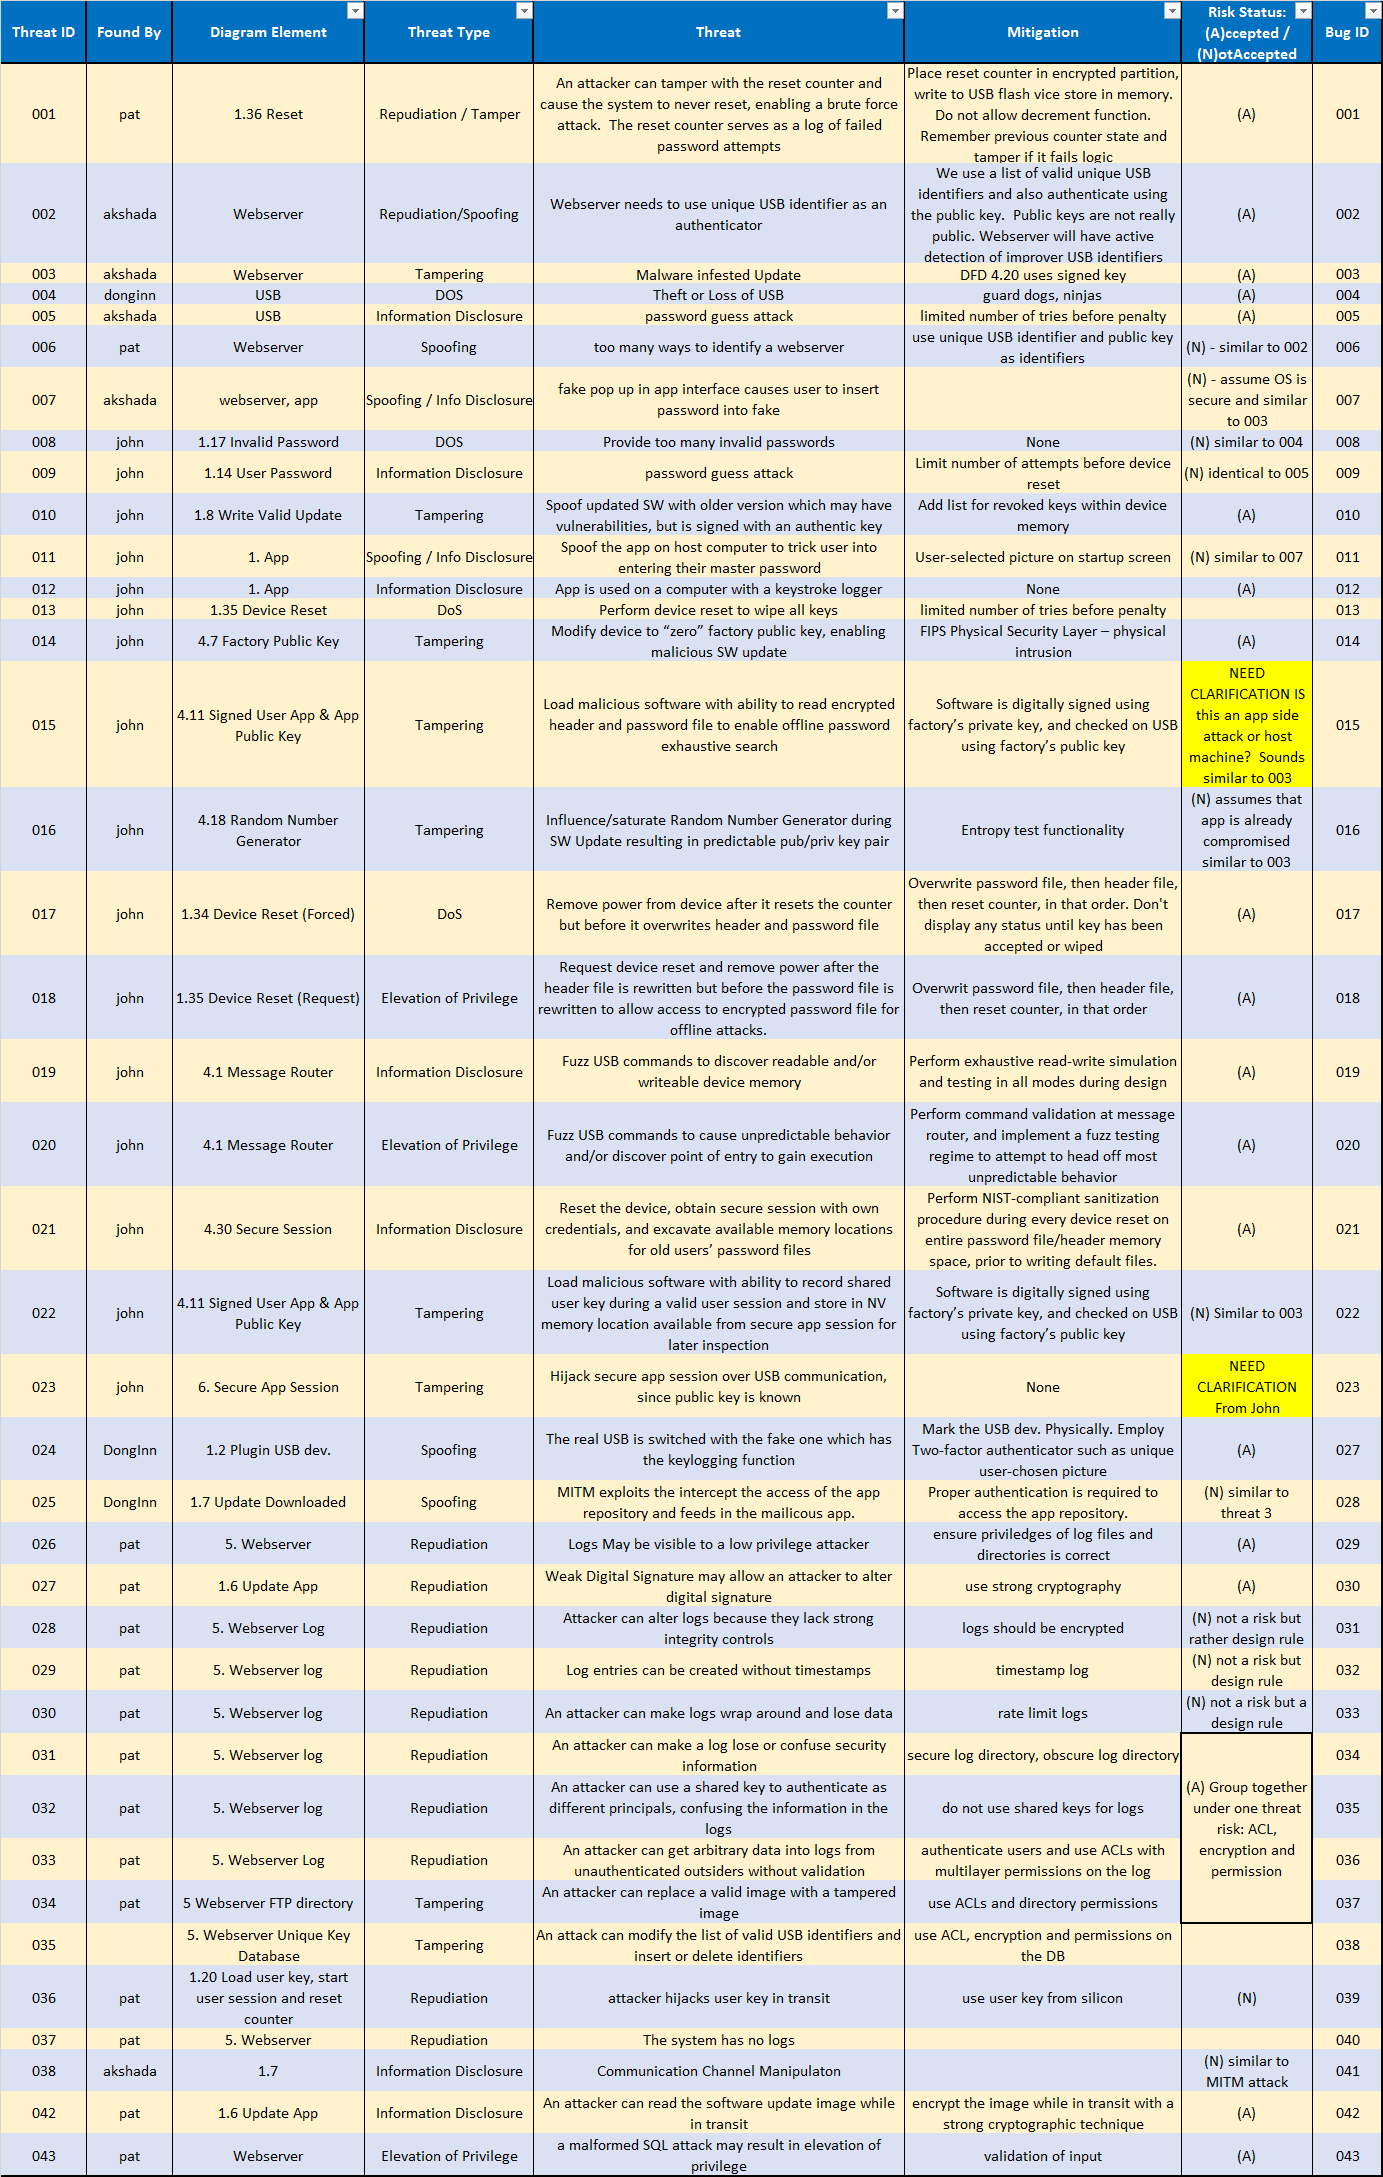
\includegraphics[width=\linewidth]{threat_list_final}
  \caption{Final Table of Threats}
  \label{tab:threatlist}
\end{table*}